
\documentclass[varwidth]{standalone}

\usepackage{tikz}
\usepackage{xcolor}
\usetikzlibrary{arrows}
\usetikzlibrary{backgrounds}
\usetikzlibrary{calc}
\usetikzlibrary{fit}
\usetikzlibrary{positioning}
\usetikzlibrary{patterns}
\usetikzlibrary{shapes}
\usetikzlibrary{shapes.misc}

\let\code=\texttt

\begin{document}

\centering

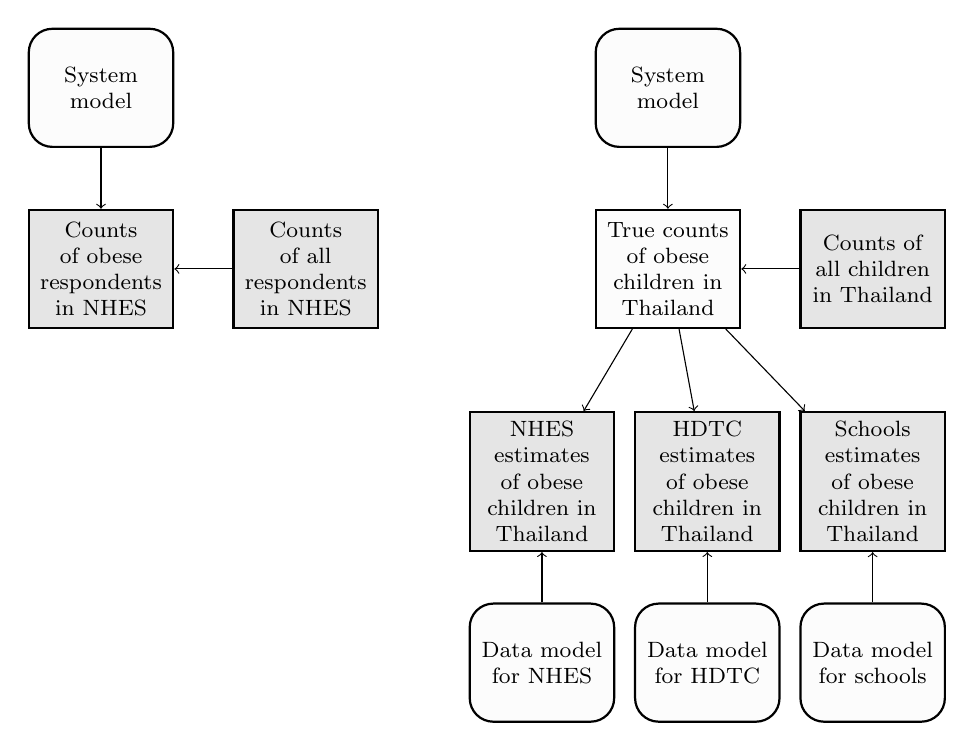
\begin{tikzpicture}
  [
    node distance = 2.1cm,
    node/.style = {thick, rectangle, draw,  text width = 1.6cm,
                   minimum height = 1.5cm,
                   font = \footnotesize, align = center},
    obs/.style = {node, fill = black!10},
    unobs/.style = {node, fill = black!1},
    model/.style = {unobs, rounded corners=0.3cm},
    label/.style = {rectangle, font = \footnotesize, align = center},
    dots/.style = {},
    arrow/.style  = {> = stealth, thick},
    arrow-out/.style = {arrow, ->},
    arrow-in/.style = {arrow, <-},
  ]
  \node[obs](counts_obs){Counts of obese respondents in NHES};
  \node[model] [above of = counts_obs, yshift = 0.2cm] (sys_mod_obs) {System model}
      edge [->](counts_obs);
  \node[obs][right of = counts_obs, xshift = 0.5cm](expose_obs){Counts of all respondents in NHES}
      edge [->](counts_obs);

  \node[unobs][right of = expose_obs, xshift = 2.5cm](counts_unobs){True counts of obese children in Thailand};
  \node[obs] [below of = counts_unobs, xshift = 0.5cm, yshift = -0.6cm] (dataset2){HDTC estimates of obese children in Thailand}
edge [<-](counts_unobs);
  \node[obs] [left of = dataset2, xshift = 0cm](dataset1){NHES estimates of obese children in Thailand}
edge [<-](counts_unobs);
  \node[obs] [right of = dataset2, xshift = 0cm] (dataset3){Schools estimates of obese children in Thailand}
edge [<-](counts_unobs);
  \node[obs][right of = counts_unobs, xshift = 0.5cm](expose_unobs){Counts of all children in Thailand}
      edge [->](counts_unobs);
  \node[model] [below of = dataset1, yshift = -0.2cm] (data_mod_1) {Data model for NHES}
edge [->](dataset1);
  \node[model] [below of = dataset2, yshift = -0.2cm] (data_mod_2) {Data model for HDTC}
edge [->](dataset2);
  \node[model] [below of = dataset3, yshift = -0.2cm] (data_mod_3) {Data model for schools}
edge [->](dataset3);
  \node[model] [above of = counts_unobs, yshift = 0.2cm] (sys_mod_unobs) {System model}
edge [->](counts_unobs);
\end{tikzpicture}

\end{document}
